\documentclass[12pt,a4paper]{article}

% ─── Page Layout ───────────────────────────────────────────────────────────────
\usepackage[a4paper, margin=0.8in, headheight=14pt]{geometry}

% ─── Fonts (XeLaTeX) ───────────────────────────────────────────────────────────
\usepackage{fontspec}
\usepackage{unicode-math}
\setmainfont{TeX Gyre Pagella}
\setmonofont[Scale=0.88]{TeX Gyre Cursor}
\setmathfont{Latin Modern Math}

% ─── Packages ──────────────────────────────────────────────────────────────────
\usepackage{xcolor}
\usepackage{colortbl}
\usepackage{titlesec}
\usepackage{enumitem}
\usepackage{tabularx}
\usepackage{booktabs}
\usepackage{array}
\usepackage{amsmath}
\usepackage{tikz}
\usetikzlibrary{shapes.geometric, arrows.meta, positioning, calc, fit, circuits.ee.IEC}
\usepackage{tcolorbox}
\tcbuselibrary{skins, breakable}
\usepackage{hyperref}
\usepackage{fancyhdr}
\usepackage{graphicx}
\usepackage{microtype}
\hyphenpenalty=10000
\exhyphenpenalty=10000
\sloppy
\usepackage{caption}
\usepackage{setspace}
\usepackage{multirow}
\usepackage{tocloft}

% ─── Q&A helper ────────────────────────────────────────────────────────────────
\newcommand{\Q}[1]{\textbf{#1}\par\noindent\ignorespaces}

% ─── Colour Palette ────────────────────────────────────────────────────────────
\definecolor{myred}{RGB}{196,30,58}
\definecolor{mydark}{RGB}{30,30,50}
\definecolor{mygreen}{RGB}{14,120,80}
\definecolor{myteal}{RGB}{0,130,140}
\definecolor{myamber}{RGB}{180,100,0}
\definecolor{mypurple}{RGB}{100,30,160}
\definecolor{mygray}{RGB}{246,247,249}
\definecolor{mgframe}{RGB}{180,185,200}
\definecolor{watermark}{RGB}{145,150,170}
\definecolor{hdrred}{RGB}{250,232,235}
\definecolor{hdrgreen}{RGB}{220,244,233}
\definecolor{hdrteal}{RGB}{220,242,244}
\definecolor{hdramber}{RGB}{253,242,215}
\definecolor{hdrpurple}{RGB}{238,228,255}
\definecolor{hdrgray}{RGB}{238,240,245}
\definecolor{rowalt}{RGB}{250,251,253}

% ─── Section Formatting ────────────────────────────────────────────────────────
\titleformat{\section}
  {\large\bfseries\color{myred}}{\thesection.}{0.5em}{}
  [\vspace{1pt}{\color{myred}\rule{\linewidth}{0.8pt}}]
\titleformat{\subsection}
  {\normalsize\bfseries\color{myteal}}{\thesubsection}{0.5em}{}
\titlespacing*{\section}{0pt}{18pt}{7pt}
\titlespacing*{\subsection}{0pt}{11pt}{4pt}

% ─── Paragraph ─────────────────────────────────────────────────────────────────
\setlength{\parindent}{0pt}
\setlength{\parskip}{4pt}

% ─── TOC Styling ───────────────────────────────────────────────────────────────
\renewcommand{\cfttoctitlefont}{\large\bfseries\color{myred}}
\renewcommand{\cftaftertoctitle}{\par\noindent{\color{myred}\rule{\linewidth}{0.8pt}}}
\setlength{\cftbeforetoctitleskip}{0pt}
\setlength{\cftaftertoctitleskip}{6pt}
\renewcommand{\cftsecfont}{\normalsize\bfseries\color{mydark}}
\renewcommand{\cftsecpagefont}{\normalsize\bfseries\color{mydark}}
\renewcommand{\cftsecleader}{\cftdotfill{\cftdotsep}}
\setlength{\cftbeforesecskip}{7pt}
\renewcommand{\cftsubsecfont}{\small\color{mydark}}
\renewcommand{\cftsubsecpagefont}{\small\color{mydark}}
\setlength{\cftbeforesubsecskip}{3pt}
\setlength{\cftsubsecindent}{1.4em}

% ─── Table helpers ─────────────────────────────────────────────────────────────
\renewcommand{\arraystretch}{1.45}
\setlength{\tabcolsep}{6pt}
\arrayrulecolor{mydark}
\newcolumntype{B}[1]{>{\small\bfseries\raggedright\arraybackslash}m{#1}}
\renewcommand{\tabularxcolumn}[1]{m{#1}}
\newcolumntype{C}[1]{>{\centering\arraybackslash}p{#1}}

% ─── Header / Footer ───────────────────────────────────────────────────────────
\pagestyle{fancy}
\fancyhf{}
\fancyhead[L]{\small\color{myred}\textbf{EC601}\;\color{mydark}— Control System}
\fancyhead[R]{\small\color{myteal}\textbf{Module 2 Notes}}
\fancyfoot[C]{\small\color{mydark}\thepage}
\fancyfoot[R]{\small\color{watermark}\textit{\copyright\ Biraj}}
\renewcommand{\headrulewidth}{0.5pt}
\renewcommand{\footrulewidth}{0.3pt}

% ─── Hyperref ──────────────────────────────────────────────────────────────────
\hypersetup{
  colorlinks=true, linkcolor=myteal, urlcolor=myteal,
  pdfauthor={Biraj Sarkar},
  pdftitle={EC601 — Module 2 Notes}
}

% ─── tcolorbox styles ──────────────────────────────────────────────────────────
\tcbset{
  tikzbox/.style={
    colback=mygray, colframe=mgframe, boxrule=0.6pt, arc=4pt,
    left=8pt, right=8pt, top=6pt, bottom=6pt,
    colbacktitle=mgframe, coltitle=mydark, fonttitle=\small\bfseries
  },
  defbox/.style={
    colback=hdrgreen, colframe=mygreen, boxrule=0.8pt, arc=4pt,
    left=9pt, right=9pt, top=6pt, bottom=6pt,
    colbacktitle=mygreen, coltitle=white, fonttitle=\small\bfseries
  },
  formulabox/.style={
    colback=hdrteal, colframe=myteal, boxrule=0.8pt, arc=4pt,
    left=9pt, right=9pt, top=7pt, bottom=7pt,
    colbacktitle=myteal, coltitle=white, fonttitle=\small\bfseries
  },
  examplebox/.style={
    colback=hdramber, colframe=myamber, boxrule=0.8pt, arc=4pt,
    left=9pt, right=9pt, top=6pt, bottom=6pt,
    colbacktitle=myamber, coltitle=white, fonttitle=\small\bfseries
  },
  masonbox/.style={
    colback=hdrpurple, colframe=mypurple, boxrule=0.8pt, arc=4pt,
    left=9pt, right=9pt, top=6pt, bottom=6pt,
    colbacktitle=mypurple, coltitle=white, fonttitle=\small\bfseries
  },
  exambox/.style={
    colback=hdrpurple, colframe=mypurple, boxrule=1pt, arc=5pt,
    left=10pt, right=10pt, top=8pt, bottom=8pt,
    colbacktitle=mypurple, coltitle=white, fonttitle=\bfseries,
    breakable
  }
}
% Allow all boxes to break across pages — prevents footer overflow
\tcbset{breakable}

% ─── TikZ styles ───────────────────────────────────────────────────────────────
\tikzset{
  block/.style={rectangle, draw=myteal, fill=hdrteal,
    text width=2.4cm, align=center, minimum height=0.95cm,
    font=\small, rounded corners=3pt, line width=0.7pt},
  wblock/.style={rectangle, draw=myteal, fill=hdrteal,
    text width=3.2cm, align=center, minimum height=0.95cm,
    font=\small, rounded corners=3pt, line width=0.7pt},
  redblock/.style={rectangle, draw=myred, fill=hdrred,
    text width=2.4cm, align=center, minimum height=0.95cm,
    font=\small, rounded corners=3pt, line width=0.7pt},
  greenblock/.style={rectangle, draw=mygreen, fill=hdrgreen,
    text width=2.4cm, align=center, minimum height=0.95cm,
    font=\small, rounded corners=3pt, line width=0.7pt},
  sumjunc/.style={circle, draw=myamber, fill=hdramber,
    minimum size=0.62cm, font=\small, line width=0.8pt},
  arrow/.style={-Stealth, thick, color=mydark},
  redarrow/.style={-Stealth, thick, color=myred},
  line/.style={thick, color=mydark}
}

% ═══════════════════════════════════════════════════════════════════════════════
\begin{document}
% ═══════════════════════════════════════════════════════════════════════════════

\begin{center}
  {\LARGE\bfseries\color{myred} EC601 — Control System}\\[5pt]
  {\normalsize\color{mydark} Semester VI \quad$\bullet$\quad 3L:0T:0P \quad$\bullet$\quad 3 Credits}\\[3pt]
  {\normalsize\color{myteal}\textbf{Module 2 Exam Notes}}\\[3pt]
  {\small\color{mydark} CGEC \;$|$\; B.Tech ECE (2023--27) \;$|$\; \textit{Biraj Sarkar}}
\end{center}
\vspace{2pt}
\noindent{\color{myred}\rule{\linewidth}{1.5pt}}
\vspace{2pt}

\hypersetup{linkcolor=mydark}
\tableofcontents
\hypersetup{linkcolor=myteal}
\newpage

%═══════════════════════════════════════════════════════════════════════════════
\section{Stability of Feedback Control Systems}
%═══════════════════════════════════════════════════════════════════════════════

Stability is the most fundamental requirement of any control system. An unstable system produces unbounded output even for a bounded input, making it practically useless.

\begin{tcolorbox}[defbox]
\textbf{BIBO Stability:} A system is \textbf{Bounded-Input Bounded-Output (BIBO) stable} if every bounded input produces a bounded output. For an LTI system, this requires all poles of the closed-loop transfer function to lie in the \textbf{left half of the $s$-plane} (i.e., have negative real parts).
\end{tcolorbox}

\subsection{Stability Conditions}

\begin{tabularx}{\linewidth}{|B{3.2cm}|X|}
\hline
\multicolumn{1}{|>{\centering\arraybackslash}p{3.2cm}|}{\textbf{\color{myteal}Condition}} &
\multicolumn{1}{>{\centering\arraybackslash}X|}{\textbf{\color{myteal}Meaning}} \\
\hline
Stable & All closed-loop poles have \textbf{negative real parts} (left half $s$-plane). Output decays to zero. \\
\hline
Marginally Stable & Poles on the \textbf{imaginary axis} (zero real part). Output oscillates with constant amplitude. \\
\hline
Unstable & At least one pole in the \textbf{right half $s$-plane}. Output grows without bound. \\
\hline
\end{tabularx}

\subsection{Relative Stability}

Absolute stability only tells us \textit{whether} a system is stable. \textbf{Relative stability} tells us \textit{how stable} — i.e., how far the closed-loop poles are from the imaginary axis.

\begin{tcolorbox}[defbox]
\textbf{Relative Stability:} A measure of the degree of stability. A system with poles far into the left half-plane is \textit{more stable} (faster decay, less oscillation) than one with poles close to the imaginary axis. Quantified by \textbf{gain margin} and \textbf{phase margin} (covered in Module 3).
\end{tcolorbox}

\begin{tcolorbox}[formulabox, title={Key Concept}]
If all poles of $T(s) = \dfrac{G(s)}{1+G(s)H(s)}$ satisfy $\text{Re}(s_i) < 0$, the system is stable.\\[4pt]
The \textbf{characteristic equation} $1 + G(s)H(s) = 0$ determines the pole locations.
\end{tcolorbox}

%═══════════════════════════════════════════════════════════════════════════════
\section{Routh–Hurwitz Stability Criterion}
%═══════════════════════════════════════════════════════════════════════════════

The Routh–Hurwitz criterion determines stability \textbf{without solving} the characteristic equation. It counts the number of roots in the right half $s$-plane using a tabular method.

\begin{tcolorbox}[defbox]
\textbf{Definition:} The \textbf{Routh–Hurwitz criterion} states that a system is stable if and only if all elements of the \textbf{first column} of the Routh array are \textbf{positive}. The number of sign changes in the first column equals the number of closed-loop poles in the right half $s$-plane.
\end{tcolorbox}

\subsection{Constructing the Routh Array}

Given the characteristic equation:
$$a_n s^n + a_{n-1}s^{n-1} + \cdots + a_1 s + a_0 = 0$$

\textbf{Step 1 — Necessary condition:} All coefficients $a_i$ must be present and have the \textbf{same sign}. If any coefficient is zero or negative, the system is \textit{unstable or marginally stable} (no need to proceed).

\textbf{Step 2 — Form the array:}

\begin{tcolorbox}[tikzbox, title={Routh Array Structure}]
\centering
\renewcommand{\arraystretch}{1.4}
\begin{tabular}{c|cccc}
$s^n$     & $a_n$     & $a_{n-2}$ & $a_{n-4}$ & $\cdots$ \\
$s^{n-1}$ & $a_{n-1}$ & $a_{n-3}$ & $a_{n-5}$ & $\cdots$ \\
$s^{n-2}$ & $b_1$     & $b_2$     & $b_3$     & $\cdots$ \\
$s^{n-3}$ & $c_1$     & $c_2$     & $c_3$     & $\cdots$ \\
$\vdots$  & $\vdots$  & $\vdots$  &           &          \\
$s^0$     & $a_0$     &           &           &          \\
\end{tabular}
\end{tcolorbox}

\begin{tcolorbox}[formulabox, title={Row Computation Formulas}]
$$b_1 = \frac{a_{n-1}\cdot a_{n-2} - a_n\cdot a_{n-3}}{a_{n-1}}, \quad
  b_2 = \frac{a_{n-1}\cdot a_{n-4} - a_n\cdot a_{n-5}}{a_{n-1}}, \quad \ldots$$
$$c_1 = \frac{b_1\cdot a_{n-3} - a_{n-1}\cdot b_2}{b_1}, \quad
  c_2 = \frac{b_1\cdot a_{n-5} - a_{n-1}\cdot b_3}{b_1}, \quad \ldots$$
Continue until all rows are complete. \textbf{Stability:} No sign changes in column 1.
\end{tcolorbox}

\subsection{Special Cases}

\begin{tabularx}{\linewidth}{|B{3.4cm}|X|}
\hline
\multicolumn{1}{|>{\centering\arraybackslash}p{3.4cm}|}{\textbf{\color{myred}Special Case}} &
\multicolumn{1}{>{\centering\arraybackslash}X|}{\textbf{\color{myred}Handling}} \\
\hline
Zero in first column & Replace zero with small $\varepsilon > 0$, complete the array, then let $\varepsilon \to 0^+$. Count sign changes. \\
\hline
Entire row of zeros & System has symmetric roots (pairs on imaginary axis or real axis). Form \textbf{auxiliary polynomial} from the row above, differentiate it, and use its coefficients to replace the zero row. \\
\hline
\end{tabularx}

\subsection{Worked Example}

\begin{tcolorbox}[examplebox, title={Example — 3rd Order System}]
\textbf{Characteristic equation:} $s^3 + 2s^2 + 4s + 8 = 0$

\textbf{Routh Array:}
\renewcommand{\arraystretch}{1.3}
\begin{center}
\begin{tabular}{c|cc}
$s^3$ & $1$ & $4$ \\
$s^2$ & $2$ & $8$ \\
$s^1$ & $b_1 = \dfrac{2\times4 - 1\times8}{2} = \dfrac{0}{2} = 0$ & $0$ \\
$s^0$ & $8$ & \\
\end{tabular}
\end{center}

$b_1 = 0$ → zero in first column → replace with $\varepsilon$, let $\varepsilon\to 0^+$.\\
First column: $1,\ 2,\ \varepsilon,\ 8$ — as $\varepsilon\to 0^+$, no sign change.\\
\textbf{Result:} Marginally stable (one pair of roots on imaginary axis at $s = \pm j2$).
\end{tcolorbox}

\begin{tcolorbox}[exambox, title={Exam Tips — Routh Criterion}]
\begin{itemize}[leftmargin=*, itemsep=3pt, topsep=0pt]
  \item \textbf{Necessary condition first:} All coefficients positive and non-zero — check before building the array.
  \item \textbf{Number of sign changes} in column 1 = number of unstable poles.
  \item \textbf{Marginal stability:} Entire row of zeros → auxiliary polynomial roots on $j\omega$-axis.
  \item \textbf{Range of $K$ for stability:} Set up array with $K$, find condition on first column $> 0$.
  \item Routh criterion gives \textit{no information} about the actual pole locations — only their count in RHP.
\end{itemize}
\end{tcolorbox}

%═══════════════════════════════════════════════════════════════════════════════
\section{Steady-State Error (SSE)}
%═══════════════════════════════════════════════════════════════════════════════

Even a stable system may not track the reference input perfectly in steady state. The \textbf{steady-state error} quantifies this residual deviation after all transients have died out.

\begin{tcolorbox}[defbox]
\textbf{Definition:} The \textbf{steady-state error} $e_{ss}$ is the difference between the desired reference input and the actual output as $t \to \infty$:
$$e_{ss} = \lim_{t\to\infty} e(t) = \lim_{s\to 0}\, s\,E(s)$$
where $E(s) = \dfrac{R(s)}{1 + G(s)H(s)}$ for a unity-feedback system.
\end{tcolorbox}

\subsection{System Type Number}

The \textbf{type number} of a system is the number of open-loop poles at the origin (i.e., the number of pure integrators in $G(s)H(s)$).

$$G(s)H(s) = \frac{K\,(1+T_1 s)(1+T_2 s)\cdots}{s^N\,(1+T_a s)(1+T_b s)\cdots}$$

Here $N$ is the \textbf{type number} (0, 1, 2, \ldots). More integrators → better steady-state tracking.

\subsection{Error Constants and SSE Formulas}

\begin{tabularx}{\linewidth}{|B{2.8cm}|>{\centering\arraybackslash}X|>{\centering\arraybackslash}X|>{\centering\arraybackslash}X|}
\hline
\multicolumn{1}{|>{\centering\arraybackslash}p{2.8cm}|}{\textbf{\color{myteal}Input}} &
\textbf{\color{myteal}Type 0} & \textbf{\color{myteal}Type 1} & \textbf{\color{myteal}Type 2} \\
\hline
Step $R(s)=\frac{1}{s}$       & $\dfrac{1}{1+K_p}$ & $0$              & $0$ \\
\hline
Ramp $R(s)=\frac{1}{s^2}$     & $\infty$           & $\dfrac{1}{K_v}$ & $0$ \\
\hline
Parabola $R(s)=\frac{1}{s^3}$ & $\infty$           & $\infty$         & $\dfrac{1}{K_a}$ \\
\hline
\end{tabularx}

\begin{tcolorbox}[formulabox, title={Error Constants}]
$$K_p = \lim_{s\to 0} G(s)H(s) \quad \text{(Position constant)}$$
$$K_v = \lim_{s\to 0}\, s\,G(s)H(s) \quad \text{(Velocity constant)}$$
$$K_a = \lim_{s\to 0}\, s^2\,G(s)H(s) \quad \text{(Acceleration constant)}$$
\end{tcolorbox}

\subsection{Steady-State Accuracy}

\begin{tcolorbox}[defbox]
\textbf{Steady-State Accuracy} is the ability of a control system to track the reference input with minimum error in steady state. It is directly related to the \textbf{type number} and the \textbf{gain} of the open-loop transfer function. Higher type number and higher gain both improve steady-state accuracy.
\end{tcolorbox}

\begin{tcolorbox}[exambox, title={Exam Tips — SSE}]
\begin{itemize}[leftmargin=*, itemsep=3pt, topsep=0pt]
  \item SSE depends on \textbf{system type} and \textbf{input type} — memorise the table above.
  \item Increasing open-loop gain $K$ reduces SSE for the same type, but may reduce stability.
  \item Adding an integrator (increasing type) eliminates SSE for lower-order inputs but risks instability.
  \item For \textbf{non-unity feedback}, use $E(s) = R(s) - C(s)$ and apply final value theorem carefully.
  \item \textbf{Final Value Theorem} valid only if $sE(s)$ has all poles in LHP (system must be stable).
\end{itemize}
\end{tcolorbox}

%═══════════════════════════════════════════════════════════════════════════════
\section{Disturbance Rejection, Sensitivity and Robustness}
%═══════════════════════════════════════════════════════════════════════════════

\subsection{Disturbance Rejection}

Real systems are subject to unwanted inputs (disturbances) such as load changes, noise, and environmental variations. A good control system must \textbf{reject disturbances} — i.e., minimise their effect on the output.

\begin{tcolorbox}[defbox]
\textbf{Disturbance Rejection:} The ability of a closed-loop system to suppress the effect of disturbance inputs $D(s)$ on the output $Y(s)$. The \textbf{disturbance transfer function} is:
$$\frac{Y(s)}{D(s)}\bigg|_{R=0} = \frac{G_p(s)}{1 + G_c(s)G_p(s)H(s)}$$
High controller gain $G_c(s)$ reduces this ratio, improving disturbance rejection.
\end{tcolorbox}

\begin{tcolorbox}[tikzbox, title={Closed Loop with Disturbance}]
\centering
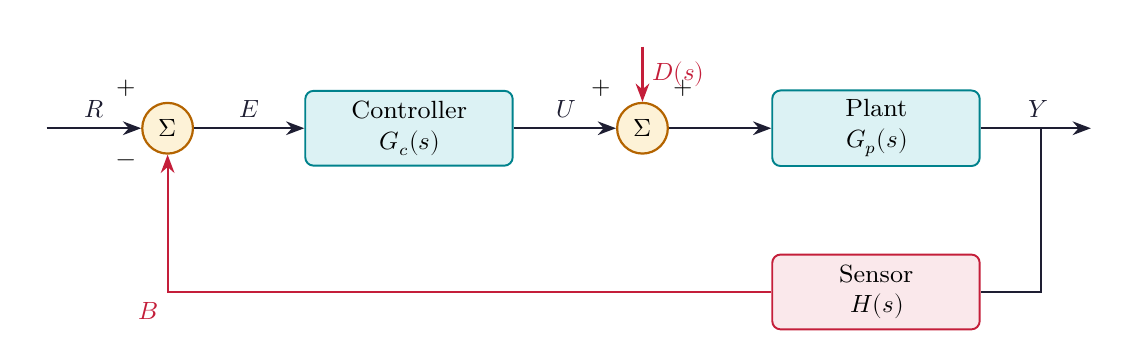
\begin{tikzpicture}[node distance=0.5cm and 1.6cm]
  \node[sumjunc] (sum1) {$\Sigma$};
  \node[block, right=1.4cm of sum1] (gc) {Controller\\$G_c(s)$};
  \node[sumjunc, right=1.3cm of gc] (sum2) {$\Sigma$};
  \node[block, right=1.3cm of sum2] (gp) {Plant\\$G_p(s)$};
  \node[redblock, below=1.1cm of gp] (H) {Sensor\\$H(s)$};
  \node[left=1.2cm of sum1] (ref) {};
  \node[right=1.4cm of gp]  (out) {};
  \node[above=0.7cm of sum2] (dist) {};

  \draw[arrow] (ref)  -- node[above]{\small $R$}   (sum1);
  \draw[arrow] (sum1) -- node[above]{\small $E$}   (gc);
  \draw[arrow] (gc)   -- node[above]{\small $U$}   (sum2);
  \draw[arrow] (sum2) -- (gp);
  \draw[arrow] (gp)   -- node[above]{\small $Y$}   (out);
  \draw[redarrow] (dist) -- node[right]{\small $D(s)$} (sum2);
  \coordinate (tap) at ($(gp.east)!0.5!(out)$);
  \draw[line]  (tap) |- (H.east);
  \draw[redarrow] (H.west) -| node[below left]{\small $B$} (sum1.south);
  \node[above left=1pt and 1pt of sum1]{\small $+$};
  \node[below left=1pt and 1pt of sum1]{\small $-$};
  \node[above left=1pt and 1pt of sum2]{\small $+$};
  \node[above right=1pt and 1pt of sum2]{\small $+$};
\end{tikzpicture}
\end{tcolorbox}

\subsection{Sensitivity}

\begin{tcolorbox}[defbox]
\textbf{Sensitivity Function} $S(s)$: Measures how much the closed-loop transfer function $T(s)$ changes relative to changes in the plant $G(s)$:
$$S(s) = \frac{1}{1 + G(s)H(s)}$$
\textbf{Complementary Sensitivity} $T(s) = 1 - S(s) = \dfrac{G(s)H(s)}{1+G(s)H(s)}$\\[4pt]
Note: $S(s) + T(s) = 1$ always. High loop gain $\Rightarrow$ $S \approx 0$ (low sensitivity).
\end{tcolorbox}

\subsection{Robustness}

\begin{tcolorbox}[defbox]
\textbf{Robustness:} The ability of a control system to maintain acceptable performance despite \textit{uncertainties} in the plant model (parameter variations, unmodelled dynamics, external disturbances). A robust system has:
\begin{itemize}[leftmargin=*, itemsep=2pt, topsep=2pt]
  \item Low sensitivity to plant parameter changes
  \item Good disturbance rejection
  \item Adequate gain and phase margins
\end{itemize}
\end{tcolorbox}

\begin{tabularx}{\linewidth}{|B{3.2cm}|X|X|}
\hline
\multicolumn{1}{|>{\centering\arraybackslash}p{3.2cm}|}{\textbf{Property}} &
\multicolumn{1}{>{\centering\arraybackslash}X|}{\textbf{\color{myamber}Open Loop}} &
\multicolumn{1}{>{\centering\arraybackslash}X|}{\textbf{\color{mygreen}Closed Loop}} \\
\hline
Sensitivity to $\Delta G$ & High — directly affects output & Reduced by factor $1+GH$ \\
\hline
Disturbance rejection & None & Good (high gain helps) \\
\hline
Robustness & Poor & Better (with proper design) \\
\hline
Bandwidth & Narrow & Wider \\
\hline
\end{tabularx}

%═══════════════════════════════════════════════════════════════════════════════
\section{PID Controllers}
%═══════════════════════════════════════════════════════════════════════════════

A \textbf{PID controller} combines three control actions — Proportional, Integral, and Derivative — to achieve fast response, zero steady-state error, and good damping simultaneously.

\begin{tcolorbox}[formulabox, title={PID Control Law (Time Domain)}]
$$u(t) = K_p\,e(t) \;+\; K_i\int_0^t e(\tau)\,d\tau \;+\; K_d\,\frac{de(t)}{dt}$$
\textbf{Transfer Function (s-domain):}
$$G_c(s) = K_p + \frac{K_i}{s} + K_d s = \frac{K_d s^2 + K_p s + K_i}{s}$$
\end{tcolorbox}

\subsection{Proportional (P) Controller}

\begin{tcolorbox}[defbox]
\textbf{P Controller:} $u(t) = K_p\,e(t)$, \quad $G_c(s) = K_p$\\[3pt]
Output is proportional to the current error. Increasing $K_p$ reduces SSE but increases overshoot and may cause instability.
\end{tcolorbox}

\begin{tabularx}{\linewidth}{|B{3.4cm}|X|}
\hline
\multicolumn{1}{|>{\centering\arraybackslash}p{3.4cm}|}{\textbf{\color{mygreen}Effect of increasing $K_p$}} &
\multicolumn{1}{>{\centering\arraybackslash}X|}{\textbf{\color{mygreen}Result}} \\
\hline
Rise time         & Decreases \\
\hline
Overshoot         & Increases \\
\hline
Settling time     & Small change \\
\hline
Steady-state error & Decreases (but never zero for Type 0) \\
\hline
Stability         & Degrades at very high $K_p$ \\
\hline
\end{tabularx}

\subsection{Integral (I) Controller}

\begin{tcolorbox}[defbox]
\textbf{I Controller:} $u(t) = K_i\int e(t)\,dt$, \quad $G_c(s) = K_i/s$\\[3pt]
Integrates the error over time. Eliminates steady-state error completely (adds a pole at origin, increasing system type by 1). However, it slows the response and can cause instability (integral windup).
\end{tcolorbox}

\subsection{Derivative (D) Controller}

\begin{tcolorbox}[defbox]
\textbf{D Controller:} $u(t) = K_d\,\dfrac{de}{dt}$, \quad $G_c(s) = K_d s$\\[3pt]
Responds to the \textit{rate of change} of error — anticipates future error. Improves damping and reduces overshoot. \textbf{Never used alone} (amplifies noise; no steady-state correction). Always combined with P or PI.
\end{tcolorbox}

\subsection{Combined PID — Effect Summary}

\begin{tabularx}{\linewidth}{|>{\bfseries\raggedright\arraybackslash}p{1.8cm}|>{\centering\arraybackslash}X|>{\centering\arraybackslash}X|>{\centering\arraybackslash}X|>{\centering\arraybackslash}X|}
\hline
\multicolumn{1}{|>{\centering\arraybackslash}p{1.8cm}|}{\textbf{Controller}} &
\textbf{Rise Time} & \textbf{Overshoot} & \textbf{Settling} & \textbf{SSE} \\
\hline
P   & Decrease       & Increase  & Small $\Delta$ & Decrease  \\
\hline
I   & Decrease       & Increase  & Increase       & Eliminate \\
\hline
D   & Small $\Delta$ & Decrease  & Decrease       & No effect \\
\hline
PI  & Decrease       & Increase  & Increase       & Eliminate \\
\hline
PD  & Decrease       & Decrease  & Decrease       & No effect \\
\hline
PID & Decrease       & Decrease  & Decrease       & Eliminate \\
\hline
\end{tabularx}

\begin{tcolorbox}[exambox, title={Exam Tips — PID}]
\begin{itemize}[leftmargin=*, itemsep=3pt, topsep=0pt]
  \item \textbf{P alone:} Always has residual SSE for Type 0 systems.
  \item \textbf{I action:} Eliminates SSE but causes \textit{integral windup} — output saturates if error persists.
  \item \textbf{D action:} Improves transient response; \textbf{never used alone} — amplifies high-frequency noise.
  \item \textbf{PID transfer function} has a zero at origin (from $K_i/s$) and two zeros from numerator.
  \item \textbf{Ziegler–Nichols method} is the standard tuning technique for PID (may appear in viva).
\end{itemize}
\end{tcolorbox}

%═══════════════════════════════════════════════════════════════════════════════
\section{Realization of PID Controllers}
%═══════════════════════════════════════════════════════════════════════════════

\subsection{Op-Amp Realization}

Op-amp circuits implement P, I, D, and PID actions using resistors and capacitors. The inverting op-amp configuration is standard.

\subsubsection*{Proportional Controller}

\begin{tcolorbox}[tikzbox, title={P Controller — Inverting Amplifier}]
\centering
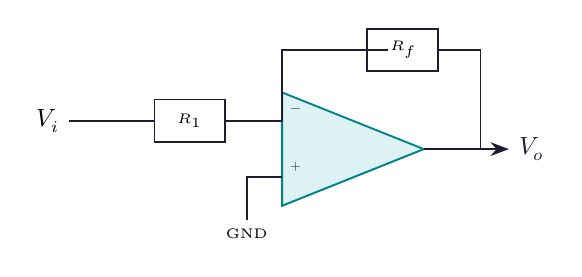
\begin{tikzpicture}[scale=0.9]
  % Op-amp symbol
  \draw[line width=0.7pt, draw=myteal, fill=hdrteal]
    (3,0) -- (3,1.6) -- (5,0.8) -- cycle;
  % Input resistor R1
  \draw[line width=0.7pt, color=mydark] (0,1.2) -- (1.2,1.2);
  \draw[line width=0.7pt, color=mydark] (1.2,0.9) rectangle (2.2,1.5);
  \node at (1.7,1.2) [font=\tiny] {$R_1$};
  \draw[line width=0.7pt, color=mydark] (2.2,1.2) -- (3,1.2);
  % Feedback resistor Rf
  \draw[line width=0.7pt, color=mydark] (3,1.2) -- (3,2.2) -- (4.5,2.2);
  \draw[line width=0.7pt, color=mydark] (4.2,1.9) rectangle (5.2,2.5);
  \node at (4.7,2.2) [font=\tiny] {$R_f$};
  \draw[line width=0.7pt, color=mydark] (5.2,2.2) -- (5.8,2.2) -- (5.8,0.8);
  % Non-inverting to ground
  \draw[line width=0.7pt, color=mydark] (3,0.4) -- (2.5,0.4) -- (2.5,-0.2);
  \node at (2.5,-0.4) [font=\tiny] {GND};
  % Output
  \draw[arrow] (5,0.8) -- (6.2,0.8) node[right,font=\small] {$V_o$};
  % Input label
  \node at (-0.3,1.2) [font=\small] {$V_i$};
  % Labels
  \node at (3.2,1.35) [font=\tiny,color=mydark] {$-$};
  \node at (3.2,0.55) [font=\tiny,color=mydark] {$+$};
\end{tikzpicture}
$$G_c(s) = -\frac{R_f}{R_1} = -K_p \qquad (K_p = R_f/R_1)$$
\end{tcolorbox}

\subsubsection*{PI Controller}

Replace $R_f$ with a series combination of $R_f$ and capacitor $C_f$:

\begin{tcolorbox}[formulabox, title={PI Controller — Op-Amp Transfer Function}]
$$G_c(s) = -\frac{Z_f}{Z_1} = -\frac{R_f + 1/(sC_f)}{R_1} = -\left(\frac{R_f}{R_1} + \frac{1}{sR_1C_f}\right) = -\left(K_p + \frac{K_i}{s}\right)$$
$$K_p = \frac{R_f}{R_1}, \qquad K_i = \frac{1}{R_1 C_f}$$
\end{tcolorbox}

\subsubsection*{PD Controller}

Replace input $R_1$ with a series combination of $R_1$ and capacitor $C_1$:

\begin{tcolorbox}[formulabox, title={PD Controller — Op-Amp Transfer Function}]
$$G_c(s) = -\frac{R_f}{R_1 + 1/(sC_1)} = -\frac{sR_fC_1}{1 + sR_1C_1} \approx -(K_p + K_d s) \text{ for small }R_1$$
$$K_p = \frac{R_f}{R_1}, \qquad K_d = R_f C_1$$
\end{tcolorbox}

\subsubsection*{PID Controller (Op-Amp)}

\begin{tcolorbox}[formulabox, title={PID Controller — Op-Amp Transfer Function}]
Use $Z_1 = R_1 + 1/(sC_1)$ as input impedance and $Z_f = R_f \| (1/sC_f)$ as feedback impedance:
$$G_c(s) = -\frac{Z_f}{Z_1} = -\frac{R_f/(1+sR_fC_f)}{R_1 + 1/(sC_1)}$$
Simplified ideal form:
$$G_c(s) = -\left(K_p + \frac{K_i}{s} + K_d s\right)$$
$$K_p = \frac{R_f}{R_1},\quad K_i = \frac{1}{R_1 C_f},\quad K_d = R_f C_1$$
The negative sign is corrected by cascading an inverting unity-gain stage.
\end{tcolorbox}

\subsection{Digital Implementation of PID}

In digital (discrete-time) systems, the PID algorithm is implemented in software using numerical approximations of integration and differentiation.

\begin{tcolorbox}[defbox]
\textbf{Discrete PID Algorithm:} With sampling period $T_s$, the continuous PID is discretised as:
\begin{itemize}[leftmargin=*, itemsep=2pt, topsep=2pt]
  \item \textbf{Proportional:} $P[k] = K_p\,e[k]$
  \item \textbf{Integral} (rectangular/trapezoidal): $I[k] = I[k-1] + K_i\,T_s\,e[k]$
  \item \textbf{Derivative} (backward difference): $D[k] = K_d\,\dfrac{e[k]-e[k-1]}{T_s}$
  \item \textbf{Output:} $u[k] = P[k] + I[k] + D[k]$
\end{itemize}
\end{tcolorbox}

\begin{tcolorbox}[formulabox, title={Pulse Transfer Function (Z-domain)}]
Using backward Euler ($s \approx \dfrac{z-1}{T_s z}$):
$$G_c(z) = K_p + K_i\frac{T_s z}{z-1} + K_d\frac{z-1}{T_s z}$$
\end{tcolorbox}

\begin{tabularx}{\linewidth}{|B{3.2cm}|X|X|}
\hline
\multicolumn{1}{|>{\centering\arraybackslash}p{3.2cm}|}{\textbf{Aspect}} &
\multicolumn{1}{>{\centering\arraybackslash}X|}{\textbf{\color{myamber}Analog (Op-Amp)}} &
\multicolumn{1}{>{\centering\arraybackslash}X|}{\textbf{\color{mygreen}Digital (Microcontroller)}} \\
\hline
Implementation  & Hardware (R, C, op-amp)       & Software (algorithm in MCU/DSP) \\
\hline
Tuning          & Change component values       & Change $K_p$, $K_i$, $K_d$ in code \\
\hline
Noise           & Susceptible to component drift & Quantisation noise; sampling delay \\
\hline
Flexibility     & Fixed once built              & Easily reprogrammable \\
\hline
Cost            & Low for simple systems        & Higher (processor needed) \\
\hline
\end{tabularx}

%═══════════════════════════════════════════════════════════════════════════════
\section{Feed-Forward Control}
%═══════════════════════════════════════════════════════════════════════════════

\begin{tcolorbox}[defbox]
\textbf{Feed-Forward Control:} A control strategy in which the controller acts on a \textit{measured disturbance} or the \textit{reference input directly}, before the disturbance affects the output. It does \textbf{not} use feedback — it anticipates and cancels the disturbance proactively.
\end{tcolorbox}

\begin{tcolorbox}[tikzbox, title={Feed-Forward + Feedback Configuration}]
\centering
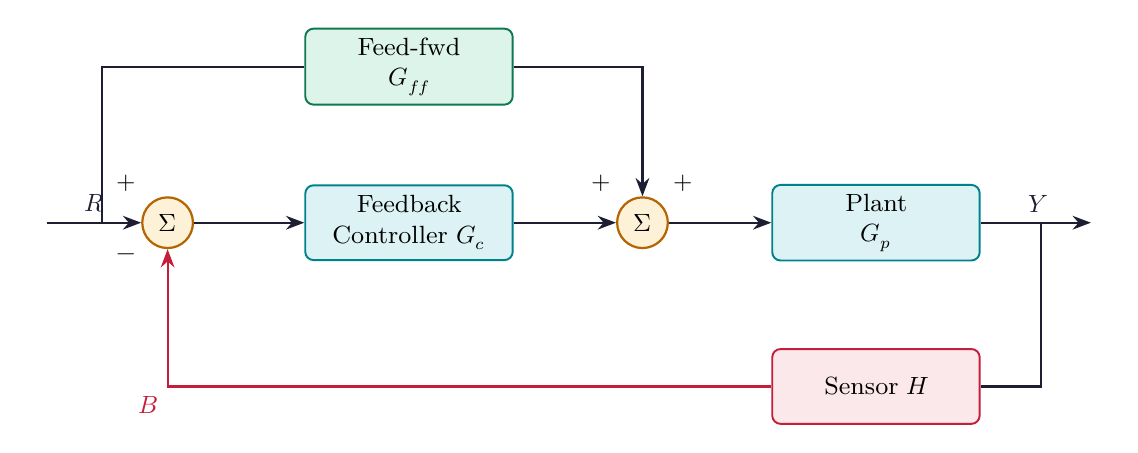
\begin{tikzpicture}[node distance=0.5cm and 1.5cm]
  \node[sumjunc] (sum1) {$\Sigma$};
  \node[block, right=1.4cm of sum1] (gc) {Feedback\\Controller $G_c$};
  \node[sumjunc, right=1.3cm of gc] (sum2) {$\Sigma$};
  \node[block, right=1.3cm of sum2] (gp) {Plant\\$G_p$};
  \node[greenblock, above=1.0cm of gc] (gff) {Feed-fwd\\$G_{ff}$};
  \node[redblock, below=1.1cm of gp] (H) {Sensor $H$};
  \node[left=1.2cm of sum1] (ref) {};
  \node[right=1.4cm of gp]  (out) {};

  \draw[arrow] (ref)  -- node[above]{\small $R$} (sum1);
  \draw[arrow] (sum1) -- (gc);
  \draw[arrow] (gc)   -- (sum2);
  \draw[arrow] (sum2) -- (gp);
  \draw[arrow] (gp)   -- node[above]{\small $Y$} (out);
  % Feed-forward path
  \coordinate (reftap) at ($(ref)!0.5!(sum1)$);
  \draw[line]  (reftap) |- (gff.west);
  \draw[arrow] (gff.east) -| (sum2.north);
  % Feedback
  \coordinate (tap) at ($(gp.east)!0.5!(out)$);
  \draw[line]  (tap) |- (H.east);
  \draw[redarrow] (H.west) -| node[below left]{\small $B$} (sum1.south);
  \node[above left=1pt and 1pt of sum1]{\small $+$};
  \node[below left=1pt and 1pt of sum1]{\small $-$};
  \node[above left=1pt and 1pt of sum2]{\small $+$};
  \node[above right=1pt and 1pt of sum2]{\small $+$};
\end{tikzpicture}
\end{tcolorbox}

\begin{tcolorbox}[formulabox, title={Ideal Feed-Forward Condition}]
For perfect disturbance cancellation, the feed-forward controller should satisfy:
$$G_{ff}(s) = -\frac{G_d(s)}{G_p(s)}$$
where $G_d(s)$ is the disturbance transfer function and $G_p(s)$ is the plant. In practice, exact cancellation is impossible due to model uncertainty — hence feedback is always retained alongside feed-forward.
\end{tcolorbox}

\begin{tabularx}{\linewidth}{|B{3.2cm}|X|X|}
\hline
\multicolumn{1}{|>{\centering\arraybackslash}p{3.2cm}|}{\textbf{Aspect}} &
\multicolumn{1}{>{\centering\arraybackslash}X|}{\textbf{\color{myamber}Feedback Only}} &
\multicolumn{1}{>{\centering\arraybackslash}X|}{\textbf{\color{mygreen}Feed-Forward + Feedback}} \\
\hline
Disturbance handling & Reacts after output is affected & Anticipates and cancels disturbance \\
\hline
Model dependency & Low (error-driven) & High (needs accurate plant model) \\
\hline
Stability risk & Inherent (loop gain) & Lower (FF is open-loop) \\
\hline
Typical use & General purpose & Known, measurable disturbances \\
\hline
\end{tabularx}

%═══════════════════════════════════════════════════════════════════════════════
\section{Multi-Loop Control Configurations}
%═══════════════════════════════════════════════════════════════════════════════

\begin{tcolorbox}[defbox]
\textbf{Multi-Loop Control:} Control architectures that use more than one feedback loop to improve performance. The most common configurations are \textbf{cascade (series)} control and \textbf{ratio control}.
\end{tcolorbox}

\subsection{Cascade (Inner–Outer Loop) Control}

\begin{tcolorbox}[defbox]
\textbf{Cascade Control:} Two feedback loops — an \textbf{inner (secondary) loop} and an \textbf{outer (primary) loop}. The output of the outer controller becomes the \textit{set-point} for the inner controller. The inner loop handles fast disturbances; the outer loop handles the primary variable.
\end{tcolorbox}

\begin{tcolorbox}[tikzbox, title={Cascade Control Block Diagram}]
\centering
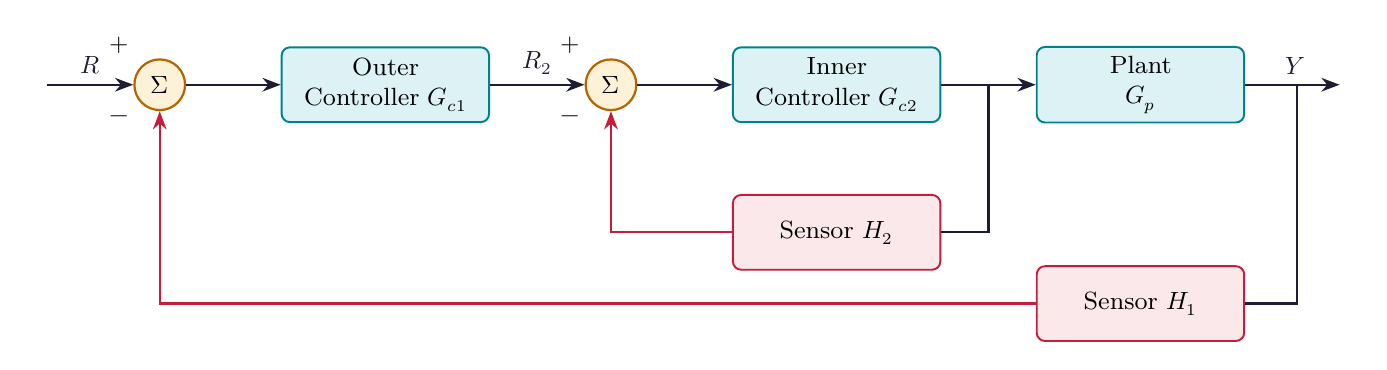
\begin{tikzpicture}[node distance=0.5cm and 1.3cm]
  \node[sumjunc] (sum1) {$\Sigma$};
  \node[block, right=1.2cm of sum1] (gc1) {Outer\\Controller $G_{c1}$};
  \node[sumjunc, right=1.2cm of gc1] (sum2) {$\Sigma$};
  \node[block, right=1.2cm of sum2] (gc2) {Inner\\Controller $G_{c2}$};
  \node[block, right=1.2cm of gc2]  (gp)  {Plant\\$G_p$};
  \node[redblock, below=0.9cm of gc2] (H2) {Sensor $H_2$};
  \node[redblock, below=1.8cm of gp]  (H1) {Sensor $H_1$};
  \node[left=1.1cm of sum1] (ref) {};
  \node[right=1.2cm of gp]  (out) {};

  \draw[arrow] (ref)  -- node[above]{\small $R$}  (sum1);
  \draw[arrow] (sum1) -- (gc1);
  \draw[arrow] (gc1)  -- node[above]{\small $R_2$} (sum2);
  \draw[arrow] (sum2) -- (gc2);
  \draw[arrow] (gc2)  -- (gp);
  \draw[arrow] (gp)   -- node[above]{\small $Y$}  (out);
  % Inner feedback
  \coordinate (tap2) at ($(gc2.east)!0.5!(gp.west)$);
  \draw[line]  (tap2) |- (H2.east);
  \draw[redarrow] (H2.west) -| (sum2.south);
  % Outer feedback
  \coordinate (tap1) at ($(gp.east)!0.5!(out)$);
  \draw[line]  (tap1) |- (H1.east);
  \draw[redarrow] (H1.west) -| (sum1.south);
  \node[above left=1pt and 1pt of sum1]{\small $+$};
  \node[below left=1pt and 1pt of sum1]{\small $-$};
  \node[above left=1pt and 1pt of sum2]{\small $+$};
  \node[below left=1pt and 1pt of sum2]{\small $-$};
\end{tikzpicture}
\end{tcolorbox}

\textbf{Advantages of Cascade Control:}
\begin{itemize}[leftmargin=*, itemsep=2pt]
  \item Inner loop rejects disturbances \textit{before} they propagate to the outer loop.
  \item Faster overall response — inner loop is tuned for speed.
  \item Outer loop can be tuned independently for accuracy.
\end{itemize}

\subsection{Ratio Control}

\begin{tcolorbox}[defbox]
\textbf{Ratio Control:} Maintains a fixed ratio between two process variables (e.g., fuel-to-air ratio in a combustion system). One variable is the \textit{wild} (uncontrolled) stream; the other is the \textit{controlled} stream adjusted to maintain the ratio.
$$\text{Set-point of controlled stream} = K_r \times \text{(measured wild stream)}$$
\end{tcolorbox}

%═══════════════════════════════════════════════════════════════════════════════
% QUICK REVISION — MODULE 2
%═══════════════════════════════════════════════════════════════════════════════
\newpage
\begin{center}
  {\large\bfseries\color{myred} Quick Revision — Module 2}\\[3pt]
  {\small\color{mydark} Feedback Control Systems $|$ EC601}
\end{center}
\noindent{\color{myred}\rule{\linewidth}{1.2pt}}
\vspace{4pt}

\begin{tcolorbox}[formulabox, title={\textbf{Key Formulas at a Glance}}]
\begin{tabularx}{\linewidth}{B{4.8cm} X}
BIBO Stability          & All closed-loop poles in LHP ($\text{Re}(s)<0$) \\[2pt]
Characteristic Equation & $1 + G(s)H(s) = 0$ \\[2pt]
Sensitivity Function    & $S(s) = \dfrac{1}{1+G(s)H(s)}$ \\[2pt]
Disturbance TF          & $\dfrac{Y}{D}\big|_{R=0} = \dfrac{G_p}{1+G_cG_pH}$ \\[2pt]
SSE (step, Type 0)      & $e_{ss} = \dfrac{1}{1+K_p}$ \\[2pt]
SSE (ramp, Type 1)      & $e_{ss} = \dfrac{1}{K_v}$ \\[2pt]
Position constant       & $K_p = \lim_{s\to0}G(s)H(s)$ \\[2pt]
Velocity constant       & $K_v = \lim_{s\to0}sG(s)H(s)$ \\[2pt]
PID (s-domain)          & $G_c(s) = K_p + K_i/s + K_d s$ \\[2pt]
PI op-amp               & $K_p = R_f/R_1,\quad K_i = 1/(R_1C_f)$ \\[2pt]
PID op-amp              & $K_p = R_f/R_1,\quad K_i = 1/(R_1C_f),\quad K_d = R_fC_1$ \\[2pt]
Digital PID integral    & $I[k] = I[k-1] + K_i T_s e[k]$ \\[2pt]
Digital PID derivative  & $D[k] = K_d(e[k]-e[k-1])/T_s$ \\[2pt]
Ideal FF condition      & $G_{ff} = -G_d/G_p$
\end{tabularx}
\end{tcolorbox}

\vspace{5pt}

\begin{tcolorbox}[defbox, title={\textbf{One-Line Definitions}}]
\begin{itemize}[leftmargin=*, itemsep=3pt, topsep=0pt]
  \item \textbf{BIBO Stability:} Bounded input $\Rightarrow$ bounded output; all CLTF poles in LHP.
  \item \textbf{Relative Stability:} How far poles are from imaginary axis; measured by gain/phase margin.
  \item \textbf{Routh Criterion:} Algebraic test for stability — no sign changes in first column of Routh array.
  \item \textbf{SSE:} Residual error as $t\to\infty$; depends on system type and input type.
  \item \textbf{System Type:} Number of open-loop poles at origin (integrators in $G(s)H(s)$).
  \item \textbf{Sensitivity:} $S = 1/(1+GH)$; measures effect of plant variation on closed-loop TF.
  \item \textbf{Robustness:} Ability to maintain performance despite model uncertainty and disturbances.
  \item \textbf{P Controller:} Proportional to error; reduces SSE but cannot eliminate it (Type 0).
  \item \textbf{I Controller:} Integrates error; eliminates SSE; risks integral windup and instability.
  \item \textbf{D Controller:} Responds to rate of change; improves damping; never used alone.
  \item \textbf{PID:} Combines all three — fast response, zero SSE, good damping.
  \item \textbf{Feed-Forward:} Acts on disturbance before it affects output; requires accurate plant model.
  \item \textbf{Cascade Control:} Inner loop handles fast disturbances; outer loop controls primary variable.
\end{itemize}
\end{tcolorbox}

\vspace{5pt}

\begin{tcolorbox}[exambox, title={\textbf{Frequently Asked / Viva Questions}}]
\begin{enumerate}[leftmargin=*, topsep=0pt, label=\textbf{Q\arabic*.}, itemsep=8pt]
  \item \Q{What is the necessary condition for stability using Routh?} All coefficients of the characteristic polynomial must be positive and non-zero.
  \item \Q{What does a sign change in Routh's first column indicate?} Each sign change corresponds to one closed-loop pole in the right half $s$-plane.
  \item \Q{What is the difference between absolute and relative stability?} Absolute: stable or not. Relative: how stable (distance of poles from imaginary axis).
  \item \Q{Why does adding an integrator eliminate SSE?} It increases system type by 1, making the velocity/position constant infinite for the corresponding input.
  \item \Q{Why is D action never used alone?} It has no DC gain ($G_c(0)=0$), cannot correct steady-state error, and amplifies high-frequency noise.
  \item \Q{What is integral windup?} When the integrator accumulates a large value during saturation, causing a large overshoot when the system comes out of saturation.
  \item \Q{What is the sensitivity function?} $S(s) = 1/(1+GH)$; measures how closed-loop TF changes with plant variation. $S+T=1$.
  \item \Q{What is the advantage of cascade control?} Inner loop rejects disturbances faster before they affect the outer (primary) loop.
  \item \Q{What is the ideal feed-forward condition?} $G_{ff} = -G_d/G_p$ — cancels disturbance perfectly (requires exact plant model).
  \item \Q{How is PID implemented digitally?} Using backward Euler or Tustin (bilinear) approximation; integral is a running sum, derivative is a backward difference.
\end{enumerate}
\end{tcolorbox}

\vspace{5pt}

\begin{tcolorbox}[tikzbox, title={\textbf{SSE Quick Reference Table}}]
\begin{tabularx}{\linewidth}{|>{\centering\arraybackslash}X|>{\centering\arraybackslash}X|>{\centering\arraybackslash}X|>{\centering\arraybackslash}X|}
\hline
\textbf{\color{myteal}Input} & \textbf{\color{myteal}Type 0} & \textbf{\color{myteal}Type 1} & \textbf{\color{myteal}Type 2} \\
\hline
Step     & $\dfrac{1}{1+K_p}$ & $0$              & $0$ \\
\hline
Ramp     & $\infty$           & $\dfrac{1}{K_v}$ & $0$ \\
\hline
Parabola & $\infty$           & $\infty$         & $\dfrac{1}{K_a}$ \\
\hline
\end{tabularx}
\end{tcolorbox}

\end{document}
